% Diese Zeile bitte -nicht- aendern.
\documentclass[course=erap]{aspdoc}
\graphicspath{ {./images/} }
\usepackage{algorithm}
\usepackage{algpseudocode}
\usepackage{amsmath,amsthm}
\usepackage{amssymb}
\usepackage[font=small,labelfont=bf]{caption}
\newcommand{\uproman}[1]{\uppercase\expandafter{\romannumeral#1}}
\newcommand{\lowroman}[1]{\romannumeral#1\relax}

%%%%%%%%%%%%%%%%%%%%%%%%%%%%%%%%%
%% TODO: Ersetzen Sie in den folgenden Zeilen die entsprechenden -Texte-
%% mit den richtigen Werten.
\newcommand{\theGroup}{142} % Beispiel: 42
\newcommand{\theNumber}{A213} % Beispiel: A123
\author{Anton Baumann \and Felix Brandis \and Michal Cizevskij}
\date{Sommersemester 2020}  % Beispiel: Wintersemester 2019/20
%%%%%%%%%%%%%%%%%%%%%%%%%%%%%%%%%

% Diese Zeile bitte -nicht- aendern.
\title{Gruppe \theGroup{} -- Abgabe zu Aufgabe \theNumber}

\usepackage{subfig}

\begin{document}
\maketitle

\section{Einleitung}
\subsection{Abstract}
Um die in der Vorlesung erlangten Kenntnisse zu vertiefen, wird vom Lehrstuhl für Rechnerarchitektur und Parallele Systeme ein Semester begleitendes Praktikum angeboten.\\
Im Rahmen dieses Rechnerarchitektur Praktikums hat sich unsere Gruppe mit dem Thema der Moore Kurve auseinandergesetzt. Die Moore Kurve ist eine von dem Mathematiker Eliakim Hastings Moore (1862-1932) entwickelte raumfüllende Kurve. Sie basiert auf der Hilbert Kurve und findet oft Anwendung in Bildverarbeitung und Datendarstellung. Unsere erste Aufgabe war es einen Algorithmus in Assembler zu entwickeln, der die Moore Kurve beliebigen Grades erstellt und in einer Datei abbildet. Die zweite Aufgabe war es zu beantworten, ob es möglich ist einen beliebigen Punkt der Kurve in konstanter Zeit unabhängig vom Grad zu berechnen.

\subsection{Charakterisierung der Moore-Kurve und weiteren raumfüllenden Kurven}
Generell ist eine raumfüllenden Kurve (Englisch: space-filling curve oder auch SFC) eine "Linie" die von einem Eindimensionalen Raum auf ein N-Dimensionalen Raum abbildet. Einfachheitshalber beschränken wir uns aber auf zweidimensionalen und ein Beispiel im dreidimensionalen Raum. Die Besonderheit dieser Kurve liegt darin, dass sie jeden Punkt des Einheitsquadrats passiert. Genauer gesagt, wenn n für den Grad der Kurve steht und $\lim_{n\to\infty}$, dann wird eine gegebene Fläche durch so eine Kurve gefüllt.\\
Die erste SFC wurde von einem Italienischen Mathematiker Giuseppe Peano in 1890 entwickelt.
\\
Die Motivation für solch eine Erkenntnis bekam er durch einen weitern  renommierten Mathematiker Georg Cantor der wenige Jahre zuvor bewiesen hatte, dass die Mengen der natürlichen Zahlen und die der positiven rationalen Zahlen gleich mächtig sind (Cantors erstes diagonal Argument)%cite ? 
Durch das verallgemeinern des Cantorischen Diagonalarguments kann man zeigen, dass es eindimensionale Objekte gibt, \\ die zweidimensionale füllen können. Eine raumfüllende Kurve ist also eine surjektive Abbildung, die von einem Einheitsintervall in ein Einheitsquadrat abbildet.
Die Hilbert Kurve, die von dem gleichnamigen Mathematiker David Hilbert in 1891 entwickelt wurde ist eine einfachere Version, die das Einheitsquadrat in 4 Teile anstatt 9 partitioniert. Diese Quadranten beinhalten dann die Hilbert Kurve vom Grad $n - 1$. \\Betrachtet man zum Beispiel die mittlere Hilbert-Kurve in Abb. \ref{fig:mooreCurve}, die den zweiten Grad hat. So bemerkt man, dass sie vier mal die Kurve vom Grad 1 beinhaltet, die rotiert oder gespiegelt wurde und an den End- bzw. Startpunkten verbunden wurden.
\begin{figure}[h]
\centering
    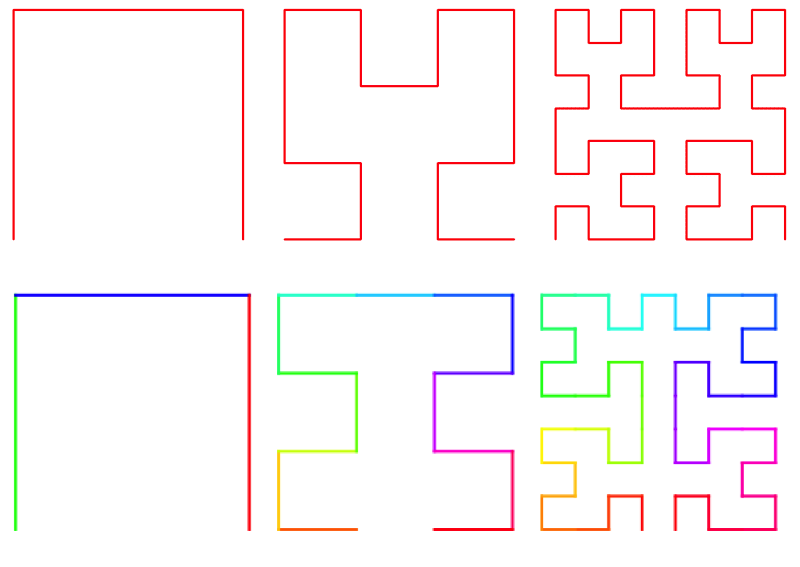
\includegraphics[width=8cm, height=5cm]{Moore_and_Hilbert}
    \caption{Die drei ersten Iterationen der Hilbert- und Moore Kurve}
    \label{fig:mooreCurve}
\end{figure}
Wie bereits erwähnt ist die Moore Kurve eine Variation der Hilbert Kurve. Die ersten Grade der Moore- und Hilbert-Kurve sind äquivalent. Dabei ergeben sich die weiteren Iterationen der Moore Kurve, durch die Zusammensetzung der Hilbert Kurve vom Grad $n - 1$.  Es werden also 4 Kopien der Hilbert Kurve des Grads $n-1$ zur Moore Kurve des Grads $n$ zusammengesetzt (Nach Rotation, Spiegelung und Verschiebung). \textbf{hier noch eine Illustration??}
Entscheidender Unterschied der Moore Kurve zur Hilbert Kurve ist, dass sich ihre Anfangs- und Endpunkte im Gegensatz zur Hilbert Kurve nebeneinander befinden.
\\
Außerdem gehört die Moore Kurve (Peano und Hilbert ebenfalls) einer Unterkategorie der SFC an, die man FASS Kurven nennt. (FASS: „space-filling, self-avoiding, simple and self-similar“).
Dies birgt wichtige Eigenschaften, weshalb sie in der Praxis Verwendung findet. Zu einem die Kurve ist selbstausweichend, das bedeutet jeder Punkt ist exakt festgelegt, also wird er nur einmal durchlaufen. Hinzu behält die Kurve die Lokalität der Punkte bei. Das bedeutet, sind die Punkte nah beinander im eindimensionalen Einheitsintervall, so sind sie es ebenfalls in der Kurve. (siehe Abb. \ref{fig:locality}) % http://blog.christianperone.com/2015/08/googles-s2-geometry-on-the-sphere-cells-and-hilbert-curve/
\begin{figure}[h]
\centering
      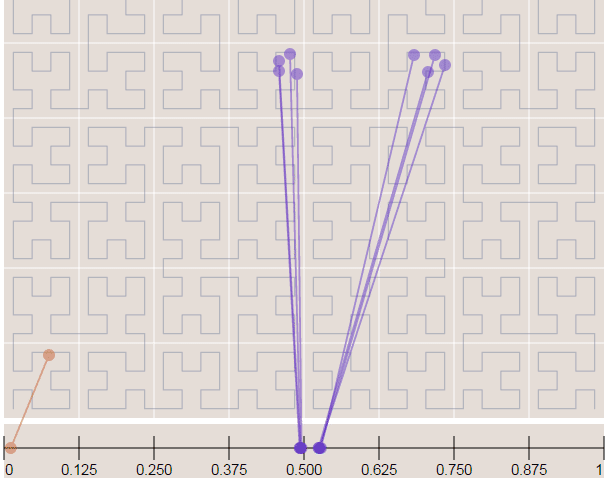
\includegraphics[width=6cm, height=4cm]{Locality}
    \caption{Graphik um die Eigenschaft der Lokalität zu verdeutlichen}
    \label{fig:locality}
\end{figure}
In raumbezogenen Anwendungen kommt es oft vor, dass raumfüllende Kurven verwendet werden, um effizient geographische Daten, die in eindimensionaler oder zweidimensionaler Form vorhanden sind, in eindimensionale Daten umzuwandeln. \\Dafür wird das Gebiet in Zellen aufgeteilt. Diese dienen einer kompakten Darstellung der bestimmten Region. Um diese Zellen schnell ansprechen zu können, werden sie indexiert. Dabei ist es erwünscht, dass geographische Nähe, also Nähe in 2 Dimensionen von Bilddaten auch auf der Abbildung in den eindimensionalen Raum erhalten bleibt, da sich so nebeneinander liegende Bilddaten auch nebeneinander im Speicher befinden und effizienter geladen werden können.
Da eine FASS Kurve genau diese Anforderungen erfüllt, eignet sie sich besonders gut für solch eine Verwendung. Ein konkretes Beispiel der Anwendung wäre die \href{https://code.google.com/archive/p/s2-geometry-library/}{S2-geometry-library von Google}. 

\begin{figure}
    \centering
    \begin{minipage}{0.45\textwidth}
        \centering
        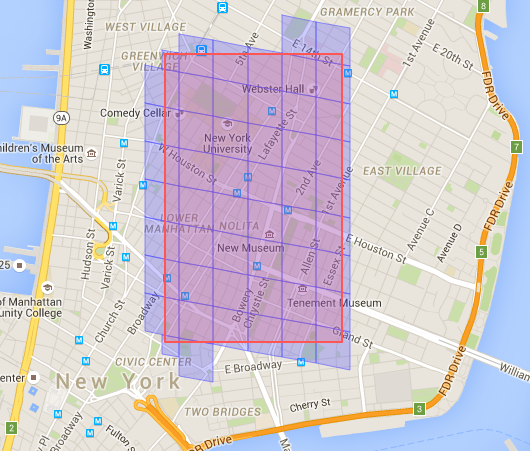
\includegraphics[width=0.9\textwidth]{Map}\\
        \caption{Einteilung von New York in Zellen}
        \label{fig:Gmaps}
    \end{minipage}\hfill
    \begin{minipage}{0.45\textwidth}
        \centering
        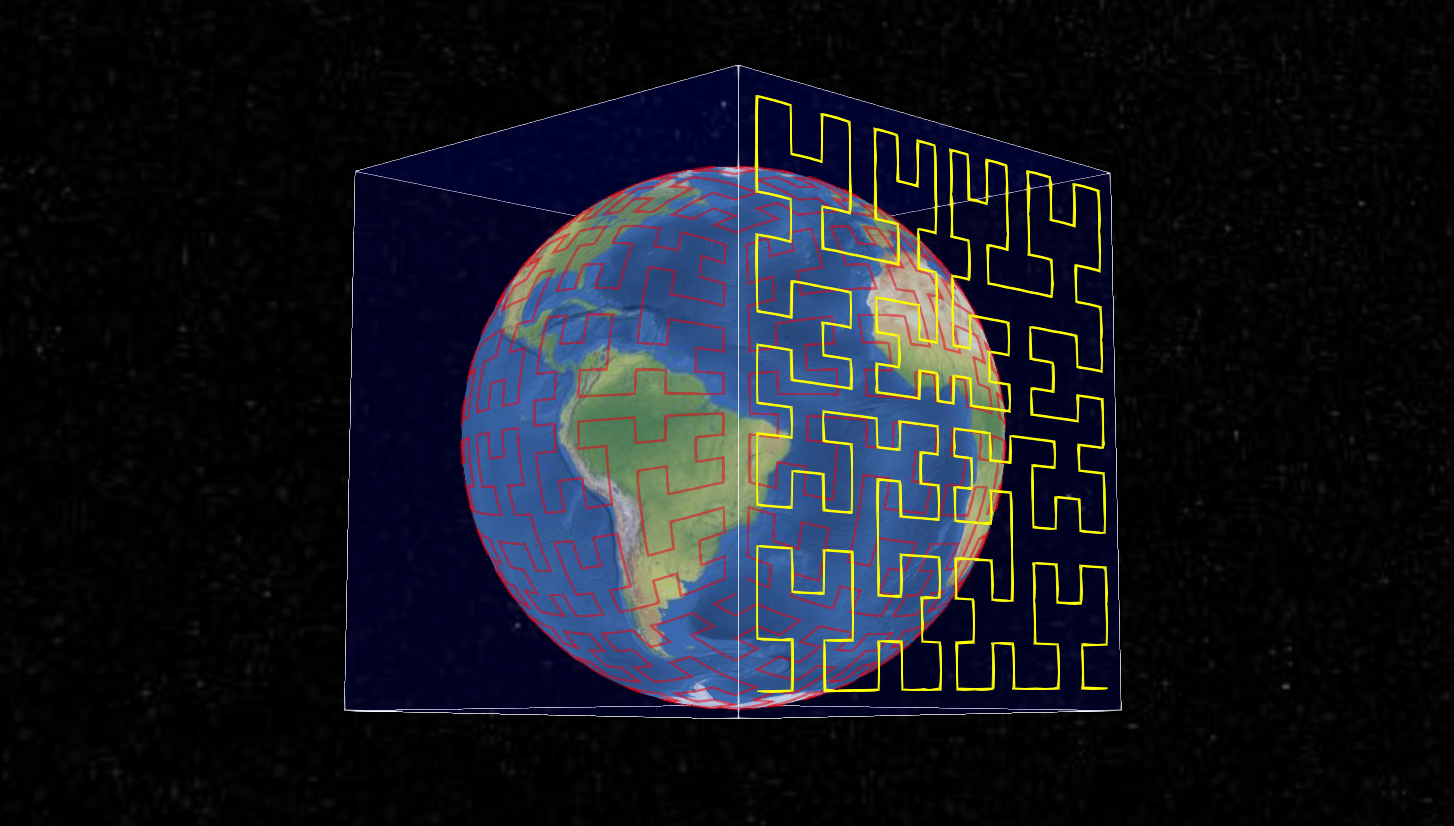
\includegraphics[width=0.9\textwidth]{Earth} \\
        \caption{Hilbert Kurve projiziert auf die Erde}
        \label{fig:hilbertCurveOnEarth}
    \end{minipage}
\end{figure}

%https://medium.com/sidewalk-talk/s2-cells-and-space-filling-curves-keys-to-building-better-digital-map-tools-for-cities-a312aa5e2f59


%\begin{center}
%   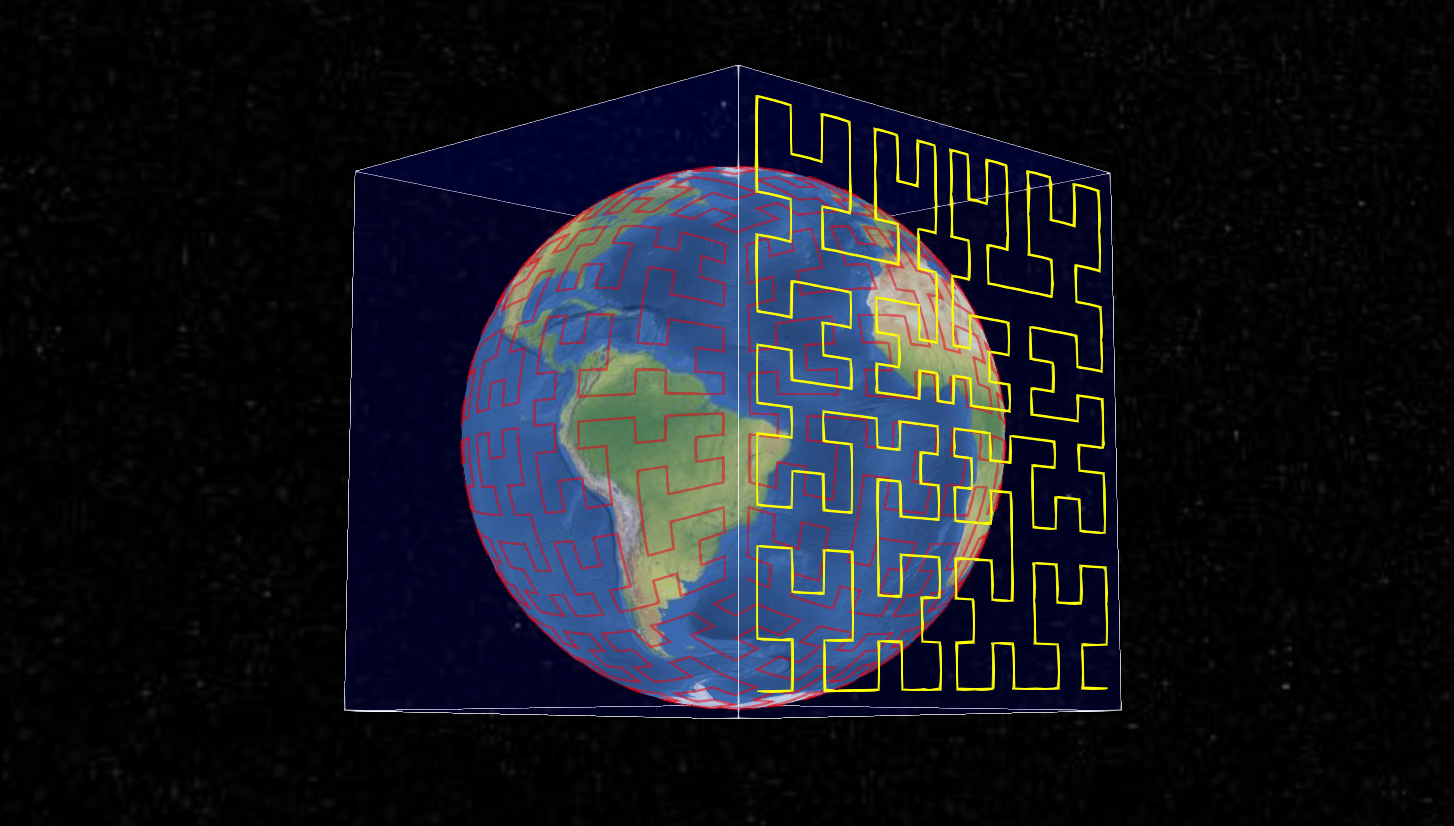
\includegraphics[width=9cm, height=6cm]{Earth}\\    %cite
%   \tiny Abbildung 6: Einteinlung der Erde 
%\end{center}


\section{Lösungsansatz}

\subsection{Die Moore Kurve}

Wie im letzten Abschnitt erwähnt, kann die Moore Kurve des Grads n aus vier Kopien der Hilbert Kurve des Grads n-1 erzeugt werden (für n > 1), siehe dazu auch Abbildung \ref{HilbertZuMoore}.
Das Problem kann also umformuliert werden in die Erzeugung der Hilbert Kurve und dem anschließendenden Kopieren, Verschieben und Rotieren der Punkte. 
\\
Es gibt rekursive Algorithmen für die Erzeugung der Hilbert Kurve, diese klammern wir im Folgenden jedoch aus. (Siehe Aufgabenstellung)

\subsection{Erzeugung der Hilbert Kurve: iterativer Punkt-für-Punkt Ansatz}
Im Folgenden soll ein Algorithmus dargestellt werden, der für gegebenen Index $i$ und Grad $n$ die Koordinaten des korrespondierenden Punktes an der Stelle $i$ der Moore Kurve berechnet.
Geht man davon aus, schon einen solchen funktionierenden Algorithmus für die Hilbert Kurve zu haben, so muss nur der Quadrant des Punktes bestimmt werden, dann der entsprechende Punkt der Hilbert Kurve errechnet und je nach Quadrant verschoben, gespiegelt oder rotiert werden. Dies wird in Abbildung \ref{HilbertZuMoore} grafisch veranschaulicht und im Algorithmus \ref{moore:iterative} skizziert.
\newline
\begin{figure}[h]
\centering
\def\svgwidth{240pt}
\input{images/HilbertZuMooreVektorG.pdf_tex}
\caption{Transformation von Hilbert Kurve des Grads n-1 zu Moore Kurve des Grads n}
\label{HilbertZuMoore}
\end{figure}
\begin{algorithm}[H]
\begin{algorithmic}
\caption{Berechne Koordinaten eines Punktes auf Moore Kurve}
\label{moore:iterative}
\Function{berechneMooreKoordinate}{$index$, $degree$}
	\State finde Quadrant $q$ des Punkts q heraus ($q \in \{A, B, C, D\}$)
	\State $tuple \leftarrow$ berechneHilbertKoordinate($index$, $degree-1$)
	\If {$q = A$} 
		\State rotiere A um 90$^{\circ} \circlearrowleft$
	\ElsIf{$q = B$}
		\State rotiere A um 90$^{\circ}\circlearrowleft$ und verschiebe nach oben
	\ElsIf{$q = C$}
		\State rotiere A um 90$^{\circ}\circlearrowright$ und verschiebe nach oben und nach rechts
	\ElsIf{$q = D$} 
		\State rotiere A um  90$^{\circ} \circlearrowright$ und verschiebe nach rechts
	\EndIf
\EndFunction
\Function{berechneHilbertKoordinate}{$index$, $degree$}
	\State [...]
\EndFunction
\end{algorithmic}
\end{algorithm}
Damit Algorithmus \ref{moore:iterative} funktioniert, fehlt noch eine Methode, die für gegebenen Index $i$ und Grad $n$ die Koordinaten des entsprechenden Punktes auf der Hilbert Kurve zurückgibt. Abbildung \ref{fig:hilbertBuildup} zeigt, wie das funktioniert: Jeder Punkt beginnt mit den Koordinatnen $(0, 0)$. Wird der Index in Binärdarstellung umgewandelt, so können von hinten beginnend immer zwei Stellen angesehen werden und dann nach dem in der Graphik dargestellten Entscheidungsmuster die Koordinaten durch Spiegelung und Verschiebung verändert werden. Durch iterative Ausführung und mit jeder Iteration einer Vergrößerung des Offsets können so die Koordinaten jedes Punktes bestimmt werden. Algorithmus \ref{hilbert:iterative} zeigt eine mögliche Formalisierung.

\begin{figure}[H] 
    \centering
    \subfloat{{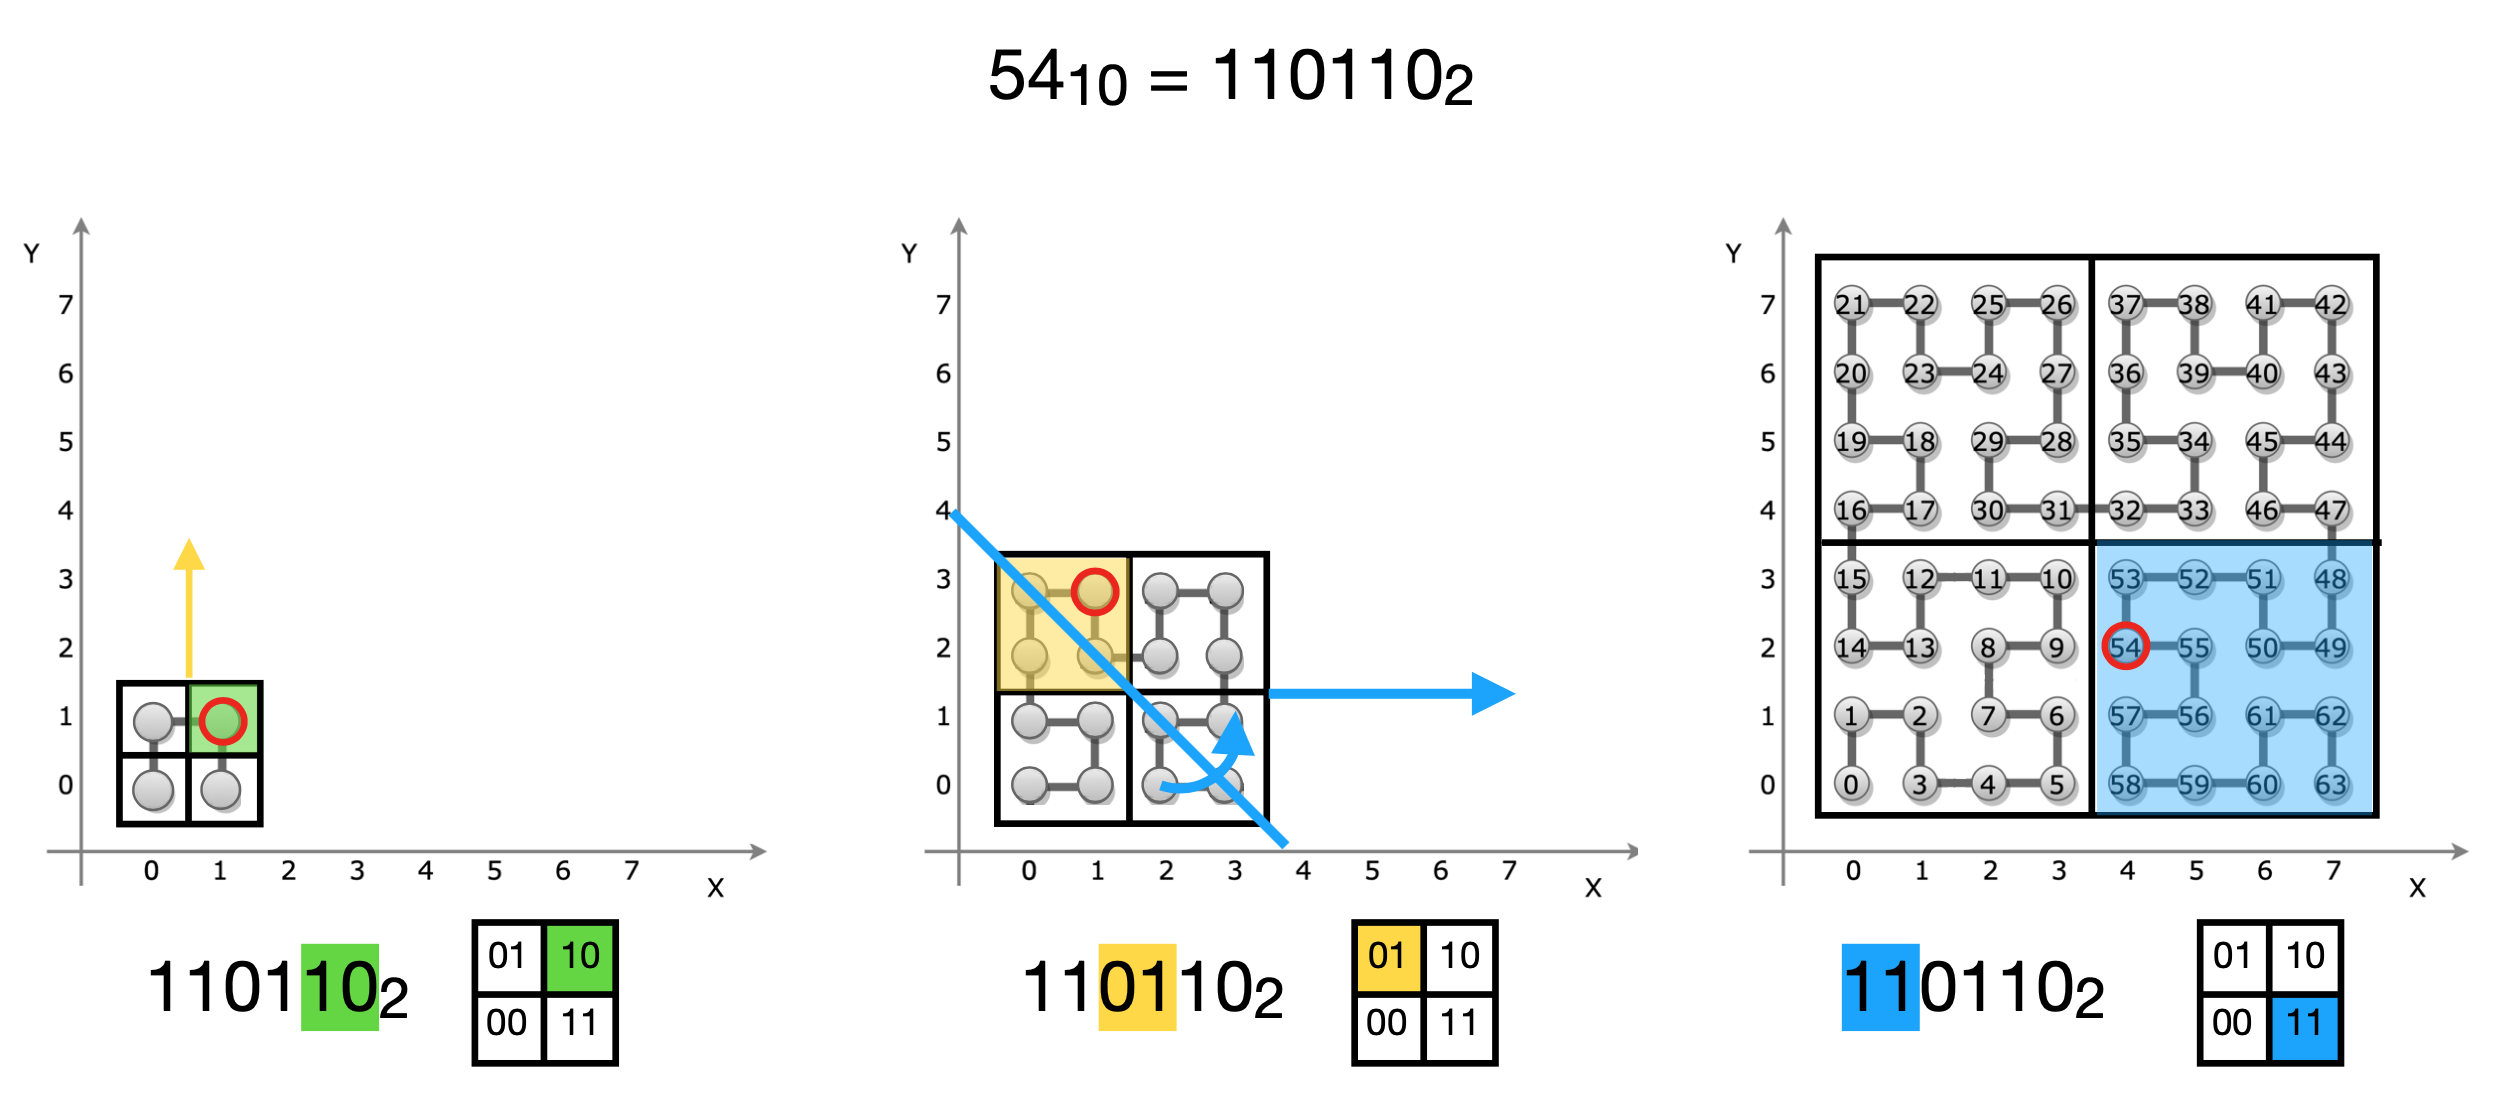
\includegraphics[width=1.0\textwidth]{HilbertToHilbert} }}%
    \caption{Bottom-up Errechnung der Koordinaten eines Punkts der Hilbert Kurve, Beispiel für Punkt mit Index 54 und HIlbert Kurve des Grads 3}%
    \label{fig:hilbertBuildup}%
\end{figure}


\begin{algorithm}[H]
\begin{algorithmic}
\caption{Berechne Koordinaten eines gegebenen Punkts auf der Hilbert Kurve}
\label{hilbert:iterative}
\Function{berechneHilbertKoordinate}{$index$, $degree$}
	\State $sidelength \leftarrow 2^{degree}$
	\State $i \leftarrow 1$
	\State $coord \leftarrow (0, 0)$
	\While {$i < sidelength$}
		\State ermittle Quadrant q $q \in \{A, B, C, D\}$ mit den letzten zwei Bits von $index$:
		\State $A \iff '00'$, $B \iff '01'$, $C \iff '10'$, $D \iff '11'$
		\If{$q \in \{A, D\}$}
			\If{$q = D$}
			\State $tmp \leftarrow coord.y$\Comment{spiegle an $y = i-1-x$ Achse}
			\State $coord.y \leftarrow i - 1 - coord.x$
			\State $coord.x \leftarrow i - 1 - tmp$	
			\Else 
			\State $swap(coord.x, coord.y)$\Comment{spiegle an $y=x$ Achse/Winkelhalbierender}
			\EndIf
		\Else 
		\State $coord.y \leftarrow coord.y + i$ \Comment{verschiebe nach oben, denn $q \in \{B, C\}$}
		\EndIf
		\If{$q \in \{C, D\}$}
		\State $coord.x \leftarrow coord.x + i$ \Comment{verschiebe nach rechts}
		\EndIf
		\State $index \leftarrow \frac{index}{4}$ \Comment{zweimaliger rechts-Bitshift um nächste 2 Bits anzusehen}
		\State $i \leftarrow 2i$\Comment{Die Seitenlänge verdoppelt sich mit jeder Iteration}
	\EndWhile
	\State \Return $coord$
\EndFunction
\end{algorithmic}
\end{algorithm}




\subsection{Erzeugung der Hilbert Kurve: Dynamischer Ansatz}
Der oben dargestellte Algorithmus hat den Vorteil, für einen gegebenen Index und Grad die Koordinaten des korrespondierenden Punktes ausrechnen zu können, ohne dafür die gesamte Kurve erzeugen zu müssen und dann die Koordinaten an der Stelle des Index auszulesen.\\ 
Soll allerdings die gesamte Kurve erstellt werden, also x-Werte und y-Werte für alle Punkte errechnet werden, so ist der iterative Aufruf des oben gezeigten Algorithmus für jeden Index sehr ineffizient.\\
Ebenso wie die Moore Kurve des Grads $n$ aus vier Kopien der Hilbert Kurve des Grads n aufgebaut werden kann, kann auch die Hilbert Kurve des Grads n aus vier Kopien der Hilbert Kurve des Grads $n-1$ erzeugt werden (Abbildung \ref{HilbertZuHilbert}).
\begin{figure}[h]
\centering
\def\svgwidth{240pt}
\input{images/HilbertZuHilbertVektorG.pdf_tex}
\caption{Transformation von Hilbert Kurve des Grads n-1 zu Hilbert Kurve des Grads n}
\label{HilbertZuHilbert}
\end{figure}
Man kann also bei der Erzeugung der Hilbert Kurve ähnlich vorgehen wie bei Algorithmus \ref{moore:iterative}: Mit gegebenen Punkten der Hilbert Kurve des Grads $n-1$ lassen sich alle Punkte der Hilbert Kurve des Grads $n$ erzeugen. 
Die Spiegelungen, Rotationen und Translationen für die jeweiligen Quadranten sind natürlich anders als in Algorithmus \ref{moore:iterative}. \\
Dieser Ansatz kann zwar keinen einzelnen Punkt an einem gegebenen Index liefern ohne die gesamte Kurve zu berechnen, andererseits ist dafür die Berechnung aller Punkte der Kurve insgesamt bei weitem effizienter als der iterative Aufruf des Punkt-zu-Punkt Ansatzes, da schon durchgeführte Berechnungen wiederverwertet werden. Algorithmus \ref{moore:batch} zeigt, wie zunächst die Hilbert Kurve bis Grad $n-1$ aufgebaut und daraus dann die Moore Kurve des Grads $n$ erzeugt wird. Für die Nachvollziehbarkeit sind Abbildung \ref{HilbertZuMoore} und \ref{HilbertZuHilbert} essentiell.
\begin{algorithm}[H]
\begin{algorithmic}
\caption{Berechne alle Punkte der Moore Kurve}
\label{moore:batch}
\Function{berechneMoorePunkte}{$degree$, int[] $x$, int[] $y$}
\State Koordinaten für $degree =1$ in Arrays hardcoden (jeweils 4 Werte)
\If {$degree = 1$}
	\Return
\EndIf	
\State berechneHilbertPunkte($degree - 1$, int[] $x$, int[] $y$)
\State $i \leftarrow 0$
\State $len \leftarrow 2^{degree - 1} -1$ \Comment{Offset für Translation}
\State $quarter \leftarrow 4^{degree-1}$\Comment{Seitenlänge der Hilbertkurve quadriert $= {(2^{degree - 1}})^2$}
\While {$i < quarter$}
\State Quadrant B: rotiere A um 90$^{\circ}\circlearrowleft$ und verschiebe um $len$ nach oben
\State Quadrant C: rotiere A um 90$^{\circ}\circlearrowright$ und verschiebe um $len$ nach oben und rechts
\State Quadrant D: kopiere C und verschiebe um $len$ nach unten
\State Quadrant A: kopiere B and verschiebe um $len$ nach unten
\State $i \leftarrow i+1$
\EndWhile
\EndFunction
\ \\
\Function{berechneHilbertPunkte}{$degree$, int[] $x$, int[] $y$}
\State $j \leftarrow 2$\Comment{Die Erzeugung beginnt bei Grad 2, da Grad 1 bereits im Speicher steht}
\State $len \leftarrow 2$ \Comment{Offset beginnt bei 2}
\State $quarter \leftarrow 4$\Comment{Algorithmus beginnt mit 4 hardgecodeten Punkten}
\While{$j \leq degree$}
\While {$i < quarter$}
	\State Quadrant B: kopiere und verschiebe A um $len$ nach oben
	\State Quadrant A: spiegle an Winkelhalbierender $x=y$
	\State Quadrant C: kopiere B und verschiebe um $len$ nach oben
	\State Quadrant D: rotiere A  um 180$^{\circ}$ und verschiebe um $len$ nach rechts
\EndWhile
\State $i \leftarrow i+1$
\State $len \leftarrow 2*len$\Comment{mit jeder Iteration verdoppelt sich die Seitenlänge..}
\State $quarter \leftarrow 4*quarter$\Comment{...und vervierfacht sich die Anzahl der Punkte}
\EndWhile
\EndFunction
\end{algorithmic}
\end{algorithm}


\subsection{Theoretische Laufzeitanalyse und Vergleich}
Bei Algorithmus \ref{hilbert:iterative} sieht man, dass der Aufwand für die Berechnung eines Punkts vom Grad der Kurve abhängt: In der $berechneHilbertKoordinate(index, degree)$ Unterfunktion wird eine Schleife $log_2(2^{degree})-1 = degree -1$ mal durchlaufen. Da der Aufwand der Operationen innerhalb der Schleife konstant ist, steigt der Aufwand für die Berechnung eines einzelnen Punkts bei Algorithmus \ref{hilbert:iterative} also linear mit dem Grad der Kurve.
\newline
Für Algorithmus \ref{moore:batch} lässt sich zeigen, dass der durschnittliche Aufwand für die Berechnung eines Punktes konstant ist, unabhängig vom Grad der Kurve. \\
Algorithmus \ref{moore:batch} besteht aus dem einmaligen Aufruf der Hilbert-Unterfunktion und dann dem Verschieben der erhaltenen Punkte zur Erzeugung der Moore Kurve. \\
In der Hilbert Unterfunktion gibt es zwei ineinander verschachtelte Schleifen: eine, die die Indexvariable $j$ von $2$ bis inklusiv  $degree -1$ durchläuft (Denn die Hilbert Unterfunktion wird ja mit $degree-1$ aufgerufen) und die innere Schleife, bei der die Punkte des letzten Grades kopiert und verschoben werden. \\ 
Diese innere Schleife wird $quarter = 4^{j-1}$ mal durchlaufen, denn es müssen immer alle Punkte der Kurve des Grads $j-1$ kopiert und verschoben werden. Diese innere Schleife hat konstanten Aufwand $c$. In ihr wird ein Punkt aus dem Speicher  geladen, die Koordinaten werden manipuliert und an 4 Stellen wieder in den Speicher geschrieben. (Die Annahme der Konstanz ist hier natürlich theoretisch: sie berücksichtigt keine Zeitunterschiede durch Caching oder RAM-Limits, sondern geht von einem idealisierten Maschinenmodell ohne die Probleme des Von-Neumann-Bottlenecks aus)\\
Nach Durchlaufen der Hilbert Unterfunktion werden in der Moore Funktion dann noch einmal  $4^{degree-1}$ Punkte kopiert und verschoben. \\ Der Aufwand für die Berechnung der Punkte der Moore Kurve des Grads n $Op(n)$ kann also folgendermaßen rekursiv definiert werden: \ \\
\[\uproman{1}: Op(n) = Op(n-1) + 4^{n-1}*\cdot\]
\[\uproman{2}: Op(1) = c\] \ \\ 
Diese rekursive Gleichung kann nun aufgelöst werden:  \ \\ 
\begin{align*}
  Op(n) &= Op(n-1) + 4^{n-1}\cdot c\\
    &= Op(n-2) + 4^{n-2}\cdot c + 4^{n-1}\cdot c \\
    &= c\cdot(4^{0} + ... + 4^{n-2} + 4^{n-1}) \\
    &= c\cdot\sum_{i=0}^{n-1} 4^{i}\\
    &= c\cdot\frac{1}{3}(4^n-1)\\
\end{align*}
Eine Kurve von Grad $n$ hat Seitenlänge $2^n$ und somit $4^n$ Punkte. Der durchschnittliche Aufwand pro Punkt $avg\_Cost(n)$ lässt sich also wie folgt berechnen: \ \\
\[avg\_Cost(n) = \frac{Op(n)}{4^n} = c \cdot \left(\frac{4^n}{3 \cdot 4^n} - \frac{1}{3 \cdot 4^n}\right) = \frac{1}{3}c - c \cdot \frac{1}{3 \cdot 4^n}\] 
\[\Rightarrow \lim_{n\to\infty} avg\_Cost(n) = \lim_{n\to\infty} \frac{Op(n)}{4^n} = \frac{1}{3}c\]  \ \\ 
Der durchschnittliche Rechenaufwand pro Punkt konvergiert also zu einem konstanten Wert. Das heißt, dass sich der absolute Aufwand bei Erhöhung des Grads um eins ungefähr um den Faktor vier erhöht, der durchschnittliche Aufwand pro Punkt aber gleich bleibt, da sich die Anzahl der Punkte mit Erhöhung des Grads ebenso vervierfacht.

% TODO: Je nach Aufgabenstellung einen der Begriffe wählen
\section{Korrektheit}
Im Gegensatz zu Aufgabenstellungen, die Floating-Point Berechnungen enthalten oder im Bereich der Kryptographie liegen, ist in unserem Fall eine Überprüfung der Korrektheit unserer Lösung zumindest in Graden <10 allein schon durch das Betrachten der visuellen Repräsentation der Koordinaten im vom Rahmenprogramm erzeugten .svg File möglich. Automatisierte Tests können lediglich die erzeugten Koordinaten mit von einer anderen Implementierung erzeugten Koordinaten abgleichen und feststellen, ob diese identisch sind, was nur bei einer bewiesen korrekten Vergleichsimplementierung aussagekräftig ist oder große Mengen an im Vorhinein gespeicherten Punktdaten erfordert.
Der Nachweis der Korrektheit der Algorithmen ist also zunächst nur durch detailliertes Nachvollziehen ihrer Funktionsweise möglich, kann aber in niedrigeren Graden sehr gut visuell überprüft werden.


\section{Performanzanalyse}
Um das Laufzeitzeitverhalten unserer Implementierung der Moore-Kurve zu überprüfen und beurteilen, haben wir Benchmarks folgender vier Implementierungen auf einem MaxBook Pro mit einem 3,1 Ghz Dual-Core Intel i7 und 16 Gb 1867 Mhz DDR3 RAM durchgeführt.

\begin{center}
    \begin{tabular}{| r | r | r | r | r | r | r |}
    \hline
    Grad \textit{n} & \# Punkte & Speicher & \textit{asm\_avx} & \textit{asm} & \textit{c\_batch} & \textit{c\_iter}  \\ \hline
    3 & 64 & 512 B  & 27 ns & 23 ns & 67 ns & 564 ns \\  \hline
    6 & 4096 & 32 KiB  & 601 ns & 1213 ns & 6524 ns & 106 $\mu s$ \\  \hline
    9 & 26144 & 2048 KiB  & 179 $\mu s$ & 289 $\mu s$ & 830 $\mu s$ & 9436 $\mu s$  \\  \hline
    12 & 16,78 * 1e6 & 128 MiB & 21,5 ms & 24,5 ms & 94,3 ms & 705,6 ms \\ \hline
    15 & 1,07 * 1e9 & 8 GiB & 1575,9 ms & 1607,4 ms & 7108,1 ms & 50759 ms \\ \hline
    16 & 4,29 * 1e9 & 32 GiB & 108,3 s & 125,7 s & 175,9 s & 442,8 s \\ \hline
    \end{tabular}
\end{center}

\begin{figure}[htbp] 
    \centering
    \subfloat[alle Implementierungen]{{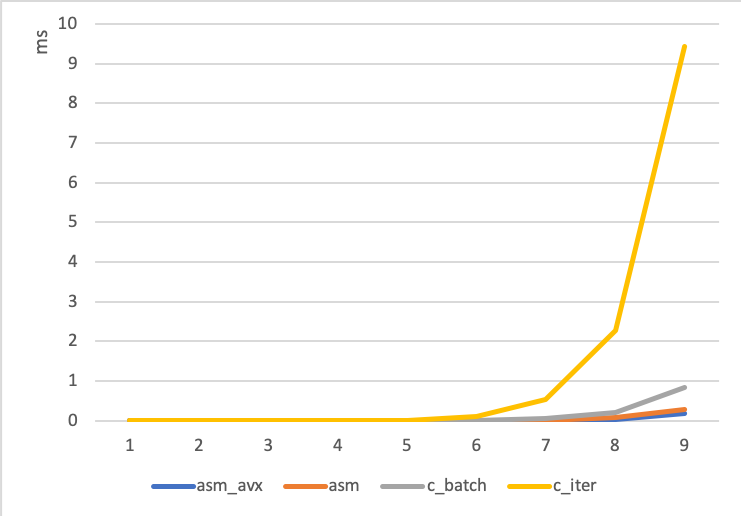
\includegraphics[width=0.45\textwidth]{laufzeit_alle_1-9.png} }}%
    \qquad
    \subfloat[ohne \textit{c\_iter}]{{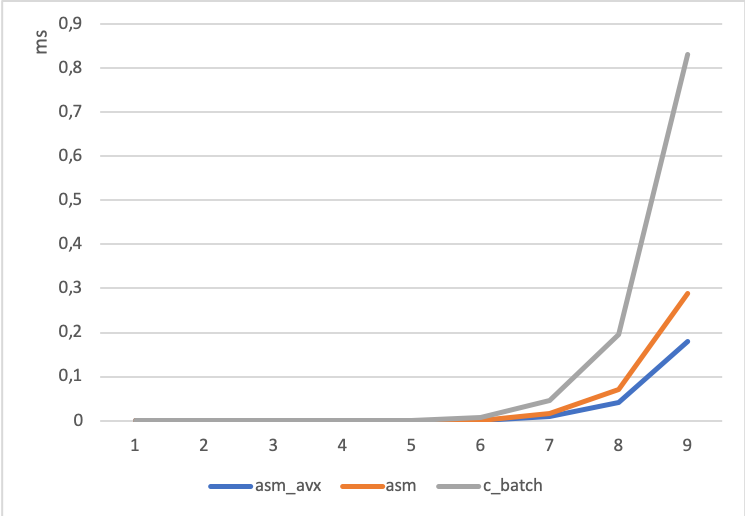
\includegraphics[width=0.45\textwidth]{laufzeit_ohne_iter.png} }}%
    \caption{Laufzeitverhalten der vier Implementierungen bis Grad 6}%
    \label{fig:Laufzeitvergleich}%
 \end{figure}
 
 \subsection{Iterative Berechnung der Moore-Koordinaten}
Aus Abb. \ref{fig:Laufzeitvergleich} geht klar hervor, dass die iterative Berechnung der Moore-Koordinaten (wie in Sektion 2 beschrieben) deutlich ineffizienter ist als die anderen Implementierungen. Ein Vorteil dieser Variante ist zwar, dass sie nur sehr wenige Speicherzugriffe benötigt, da alle Berechnungen in den Registern durchgeführt werden können und nur das Endergebnis in den Speicher geschrieben wird. Durch das rein iterative Vorgehen kann dieser Algorithmus jedoch nicht sinnvoll auf Datenebene parallelisiert werden. Auch kann der dynamische Ansatz, von dem die übrigen Implementierungen profitieren, hier nicht angewandt werden. Im folgenden liegt daher der Fokus auf den restlichen Implementierungen.

\subsection{Vergleich Assembler- mit Referenzprogramm}
Die Implementierungen \textit{c\_ batch}, \textit{asm\_avx} und \textit{asm} ... siehe Section 3 ... \newline
An Abb. \ref{fig:Laufzeitvergleich}.b und den Benchmarkwerten kann man erkennen, dass die Assembler Implementierungen deutlich performanter sind als die C-Referenzimplementierung. Für Grad 6 ist die Assembler-Implementierung, welche 128-bit Register benutzt, drei mal schneller als das C-Programm. Dies ist darin begründet, dass sich die dynamische Berechnung der Hilberkurve optimal durch SIMD parallelisieren lässt. Somit können einige Koordinaten gleichzeitig innerhalb einer Operation verarbeitet werden. Die Anzahl der Punkte, die in ein SIMD-Register passen ist abhängig vom Datentypen der Koodinaten und der Größe der Vektorregister. Wir haben uns entschieden, von der in der Aufgabenstellung vorgegebenen Signatur \texttt{moore(uint64\_t degree, uint64\_t *x, uint64\_t *y)} abzuweichen und 32 bit Integer zu benutzen. Der maximale darstellbare Wert verringert sich dadurch zwar auf $2^{32}-1$, jedoch werden größere Werte erst ab einem $n > 32$ benötigt. Der Speicherbedarf einer Moore Kurve mit Grad 33 betrüge $4^{33} \cdot 2 \cdot 4 \text{ Bytes } \approx 590 \cdot 10^{18} \text{ Bytes}$, wenn man alle Koordinaten als 32 bit unsigned Integers darstellen könnte und das Doppelte bei Benutzung von 64 bit Integern. 
\newline
Durch die Reduzierung auf 32 bit Intger können nun bei Verwenung von 128 bit Vektorregistern vier und bei 258 bit Registern acht Werte gleichzeitig verarbeitet werden (siehe Abb. 2).

\begin{figure}[htbp] 
    \centering
    \subfloat{{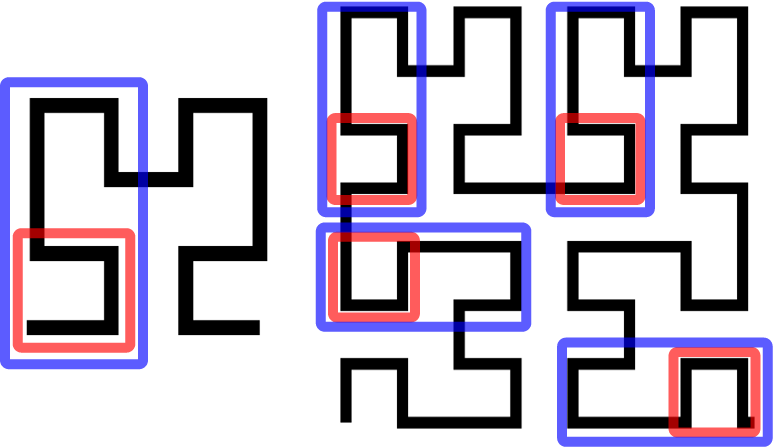
\includegraphics[width=0.69\textwidth]{hilbert_transformation.png} }}%
    \caption{Parallelisierung durch SIMD}%
    \label{fig:SIMD}%
\end{figure}

Durch Disassemblieren der mit \texttt{-march=native -O3} kompilierten Binärdatei festgestellt haben, dass der Compiler den C Code nicht vektorisiert. Daher war unsere anfängliche Vermutung, dass \textit{asm\_128} etwa vier mal so schnell ist wie unsere C-Implementierung und \textit{asm\_256} in der Hälfte der Zeit von \textit{asm\_128} terminiert.

\begin{figure}[htbp] 
    \centering
    \subfloat[Speedup Assembler- ggü. C-Implementierung]{{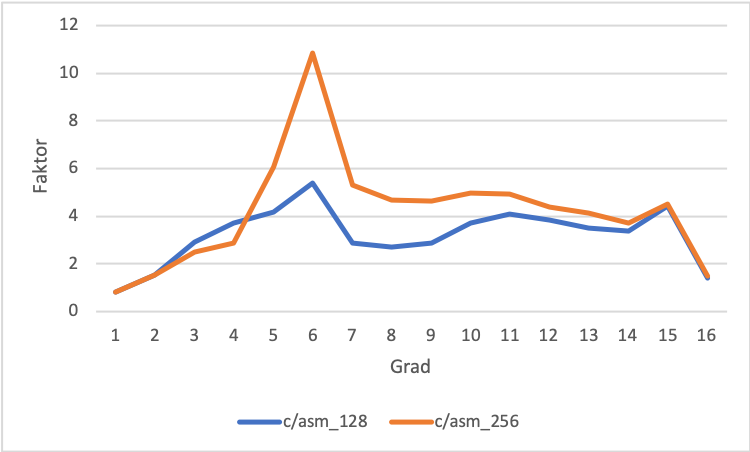
\includegraphics[width=0.45\textwidth]{speedup_base_c.png} }}%
    \qquad
    \subfloat[Speedup \textit{asm\_256} ggü. \textit{asm\_128}]{{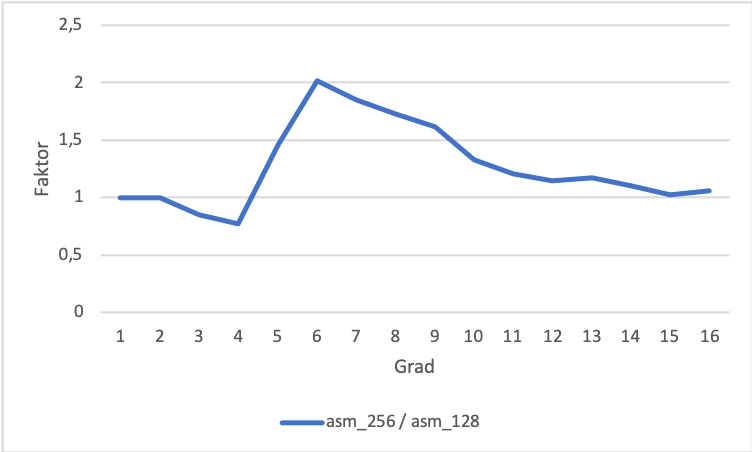
\includegraphics[width=0.45\textwidth]{speedup_base_asm_128.png} }}%
    \caption{Laufzeitvergleich C/ASM}%
    \label{fig:Laufzeitvergleich Speedup}%
 \end{figure}
 
 Abb. \ref{fig:Laufzeitvergleich Speedup}.a bestätigt den ersten Teil unserer Vermutung. Zwischen Grad 4 und 15 ist die \textit{asm\_128} Implementierung 2,8 bis 5,3 mal schneller als die Referenzimplementierung in C. Der zweite Teil trifft nur teilweise zu. Wie in Abb. \ref{fig:Laufzeitvergleich Speedup}.b zu sehen ist, profitieren vor allem Grade zwischen 6 und 10 von den größeren Vektorregistern. Bei größeren Graden bietet die Verwendung von AVX-Registern keine signifikante Performanzsteigerung.
 
\subsection{Cache Effizienz}
Abb. \ref{fig:Laufzeitvergleich Speedup}.a wirft die Frage auf, weshalb die Assembler Implementierug bei Grad 6 besonders performant ist. Dies lässt sich vermutlich damit beantworten, dass die Moore Kurve sechsten Grades genau \textit{32 KiB} an Speicher benötigt und die Größe des L1 Caches der Maschine auf der getestet wurde \textit{32 KiB} beträgt. Um diese Annahme zu überprüfen wurde das Programm mit dem MacOS Tool \textit{Instruments} auf Cache-Misses (insbesondere L1) überprüft, mit dem Ergebnis, dass 6 der höchste Grad ist, bei dem noch nahezu keine L1 Misses auftreten.

\begin{figure}[htbp] 
    \centering
    \subfloat[Grad 1 - 15]{{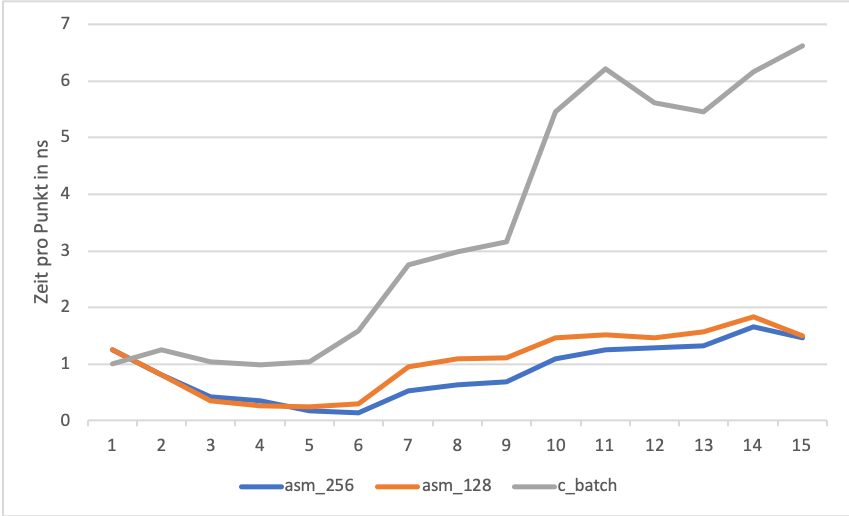
\includegraphics[width=0.45\textwidth]{ns_per_coord_1-15.png} }}%
    \qquad
    \subfloat[Grad 1 - 16]{{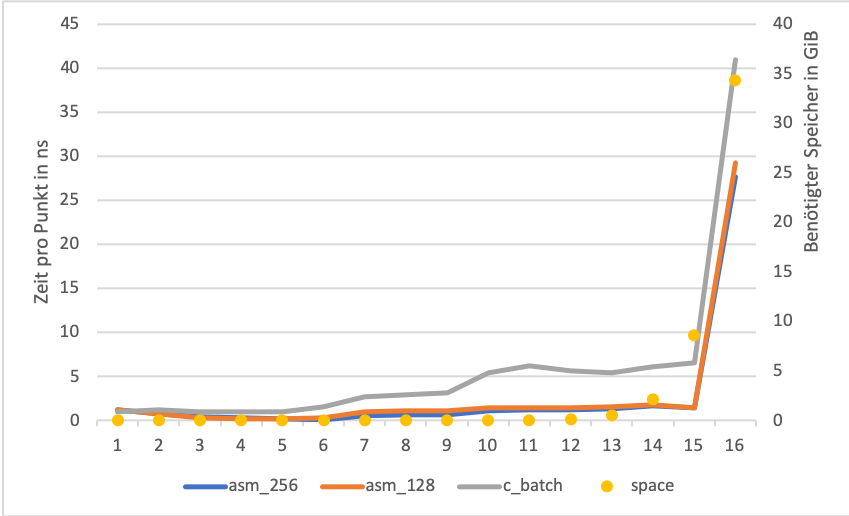
\includegraphics[width=0.45\textwidth]{ns_per_coord_1-16.png} }}%
    \caption{Nanosekunden pro Punkt der Moore Kurve}%
    \label{fig:Laufzeitvergleich Skaliert}%
 \end{figure}
 
 Der Vollständigkeit halber muss noch der Effizienzeinbruch bei Grad 16 angesprochen werden. Dieser ist damit zu erklären, dass die Speicheranforderung für die Berechnung der Moore Kurve auf 32GiB steigt. Da unser Computer nur 16 GiB an Arbeitsspeicher zur Verfügung stellt, müssen nun häufig Speicherseiten auf die Festplatte ausgelagert werden, was zu starken Performanzeinbußen führt.



\section{Zusammenfassung und Ausblick}

Selten gibt es einen Punkt, ab dem man mit Sicherheit die Möglichkeit weiterer Performanceoptimierungen eines Programms ausschließen kann. Besonders beim Schreiben von Assemblycode können so viele Faktoren wie ein simpler Tausch der Reihenfolge zweier Befehle die Schnelligkeit des Programms beeinflussen, sodass die Annahme eines voll optimierten Programms nie getroffen werden kann. \\
Nach wachsender Einarbeitung in die Thematik und Entwicklung und ständiger Verbesserung unserer Algorithmen fallen uns zu diesem Zeitpunkt noch weitere mögliche Wege der Optimierung ein.\\
Unsere Benutzung von 32-Bit Integern statt 64-Bit-Integern zur Darstellung der Koordinaten hat zu einer höheren Parallelisierbarkeit des Programms geführt. Mit hoher Wahrscheinlichkeit kann für Grade $\leq 16$ die dynamische Anpassung der Datenbreite auf 16 Bit zu einem weiteren Performancegewinn führen. In Verbindung mit der Benutzung noch breiterer Register, zum Beispiel 512 Bit AVX Registern können Berechnungen noch stärker parallelisiert werden, wobei sich die  Limitierung derartiger Optimierungen schon bei der Erhöhung von 128 Bit auf 256 Bit gezeigt hat, mit teilweise kaum besserer Perfomanz trotz breiterer Register. \\
Auch das Experimentieren mit einer veränderten Datenstruktur, also dass $x$ und $y$ Koordinaten zum Beispiel nebeneinander im gleichen Array stehen, könnte in bestimmten Fällen die Performance durch eine verbesserte Reihenfolge von Lade- und Schreibbefehlen auf den Speicher erhöhen. \\
All dies kann in unserer Herangehensweise jedoch nur den konstanten Aufwand pro Punkt verringern. Dass die Laufzeit des Algorithmus mit Erhöhung des Grads exponentiell steigt, ändert auch eine Verringerung dieser Konstante nicht und ist durch die exponentiell wachsende Punktanzahl bedingt.

%Um unsere Laufzeit zu verbessern würden wir vorschlagen, dass man unser Programm auf einem Rechner laufen lassen sollte der über mehr Arbeitsspeicher und größeren Cache verfügt, damit man Kurven von größeren Grad mit weniger Page-Faults und Cache Misses berechnen kann, was zur kürzeren Laufzeit führen würde.
%Ein weiterer Vorschlag von unserer Seite sei die Datenstruktur auf der wir arbeiten so anzupassen. Zur zeit arbeiten wir auf zwei Arrays einem X-Array und Y-Array diese liegen nacheinander im Speicher, unsere Idee ist, die Arrays folgend zu kombinieren XY-Array: x1,y1,x2,y2,….,xn,yn
%sodass man kleinere Sprünge macht beim hin und her kopieren. 


% TODO: Fuegen Sie Ihre Quellen der Datei Ausarbeitung.bib hinzu
% Referenzieren Sie diese dann mit \cite{}.
% Beispiel: CR2 ist ein Register der x86-Architektur~\cite{intel2017man}.
\bibliographystyle{plain}
\bibliography{Ausarbeitung}{}

\end{document}
